\documentclass{article}

\usepackage{uni-notes-eng}

\begin{document}
    \textbf{ZAD 1.}
    \medskip

    Mamy ułamek okresowy, czyli
    $$512,(35)=512,353535353535...$$

    Rozpisując rzędy wielkości w tym ułamku

    \begin{center}
        \begin{tabular}{ | c | c | c | c | c | c | c | c | c | }
            \hline
            100 & 10 & 1 & - & 0,1 & {\color{acc}0,01} & 0,001 & ...\\

            \hline

            5 & 1 & 2 & , & 3 & {\color{acc}5} & 3 & ... \\
            \hline
        \end{tabular}
    \end{center}

    Zaokrąglanie do części setnych oznacza, że część z $0,01$ chcemy jeszcze zachować, ale już następne cyfry nie są nam potrzebne, więc je ucinamy. Dostajemy $512,35$, ale musimy jeszcze popatrzeć co się dzieje dalej w tym ułamku. Jeżeli za miejscem gdzie ucieliśmy byłaby cyfra co najmniej $5$, to musimy zwiększyć nasz ułamek o $0,01$ (czyli dostalibyśmy $512,36$). Na szczęście, w tym konkretnym przypadku mamy
    $$512,35|3...$$
    a więc ucieliśmy przed cyfrą mniejszą od $5$, więc zostaje odpowiedź
    $$C.\; 512,35$$

    \textbf{ZAD 2.} OK
    \bigskip

    \textbf{ZAD 3.}
    \begin{align*}
        {(-2a^3b^2)^2\over -4ab^2}={(-2)^2(a^3)^2(b^2)^2\over -4ab^2}={4a^6b^4\over -4ab^2}=-\frac44{a^{6-1}b^{4-2}}=-a^5b^2=-(-2)^5\Big(-\frac14\Big)^2={2^5\over (2^2)^2}={2^5\over 2^4}={\color{acc}2:\; A.}
    \end{align*}
    
    \textbf{ZAD 4.} OK
    \bigskip

    \textbf{ZAD 5.}
    \medskip

    Dostajemy poniższą zależność:
    \begin{align*}
        \begin{matrix}
            4\;x\;JABLKA & + & 3\;x\;BRZOSKIWNIE & -- & 29,60\\
            3\;x\;JABLKA & + & 4\;x\;BRZOSKIWNIE & -- & 31,30
        \end{matrix}
    \end{align*}
    Pomnóżmy pierwsze równanie przez $4$, a drugie przez $3$:
    \begin{align*}
        \begin{matrix}
            16\;x\;JABLKA & + & 12\;x\;BRZOSKIWNIE & -- & 118,60\\
            9\;x\;JABLKA & + & 12\;x\;BRZOSKIWNIE & -- & 93,90
        \end{matrix}
    \end{align*}

    Zauważamy, że różnica między pierwszym a drugim odpowiada cenie $7$ kg jabłek, które kosztowałyby $118,60-93,90=24.5$, czyli cena jednego kg jabłek to ${24,5\over7}=3,5: A$.
    \bigskip

    \textbf{ZAD 6.} OK
    \bigskip

    \textbf{ZAD 7.}
    \medskip

    \begin{center}
    \begin{tabular}{| c | c |}
        \hline

        JERZYK & $2500{m\over min}={2500{m\over \frac1{60}h}}=2500\cdot60{m\over h}=150{km\over h}$
        
        \\
        \hline
        ZAJĄC & $20{m\over s}=20{m\over \frac1{3600}h}=20\cdot3600{m\over h}=72{km\over h}$
        
        \\
        \hline
        KOŃSKA MUCHA & $120{km\over h}$
        
        \\
        \hline
        PANTERA & $1,1{km\over min}=1,1{km\over \frac1{60}h}=66{km\over h}$
        
        \\
        \hline
    \end{tabular}
    \end{center}

    Czyli najszybszy jest jerzyk - A.
    \bigskip

    \textbf{ZAD 8.}
    \medskip

    \begin{center}
        \begin{tikzpicture}
            \draw[thick, ->](-4, 0)--(6.5, 0);
            \node at (-3.5, 0) {$\color{def}\bullet$};
            \node at (-3.5, -0.5) {$A=-7$};
            \node at (5.5, 0) {$\color{def}\bullet$};
            \node at (5.5, -0.5) {$B=11$};
            \node at (0, 0) {$\bullet$};
            \node at (0, -0.5) {$0$};
        \end{tikzpicture}
    \end{center}

    Odległość między $A$ a punktem $0$ to $|-7|=7$, a między $0$ a punktem $B$ - $|11|=11$. W takim razie odległość między $A$ a $B$ to suma tych odległości, bo leżą po dwóch osobnych stronach punktu $0$, czyli
    $$|AB|=7+11=18\neq 11-|-7|=11-7=4{\color{def}:\;F.}$$
    a jeśli byłyby po tej samej stronie, to zawsze zadziała wzór
    $$|AB|=B-A,$$
    czyli od najbardziej prawego punktu odejmujemy punkt najbardziej lewy.
    \medskip

    Skoro już wiemy, że odległość między tymi punktami to $18$, możemy podzielić ją na pół, otrzymując ${18\over2}=9$. To daje nam odległość środka od dowolnego z krańców, czyli środek to punkt o współrzędnych
    $$-7+9=2=11-9{\color{acc}:\;P.}$$

    \textbf{ZAD 9.}
    \medskip

    \begin{center}
        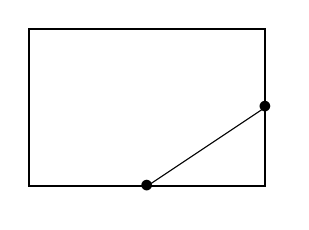
\begin{tikzpicture}
            \draw[thick] (0, 0) rectangle (3, 2);
            \node (A) at (1.5, 0) {$\bullet$};
            \node (B) at (3, 1) {$\bullet$};
            \draw(1.5, 0)--(3, 1);
        \end{tikzpicture}
    \end{center}
    To nie jest oś symetrii - oś symetrii powinna dzielić prostokąt na dwie identyczne, ale odbite jak w lustrze, części. Tutaj zostawiam znalezienie odpowiedzi Tobie - narysuj 3 prostokąty i zaznacz sytuację z podpunktów A, B i D i przekonaj się która daje oś symetrii.
    \bigskip

    \textbf{ZAD 10.}
    \medskip

    Odpowiedź $B$ odpada od razu, bo mimo że pole się zgadza, to jednak $2$ jest liczbą pierwszą, nawet jedyną liczbą pierwszą parzystą. W odpowiedzi $A$ odpada liczba pierwsza $5$, w odpowiedzi $D$ odpada liczba $1$, która nie jest ani pierwsza ani złożona. Zostaje nam więc $C$ i faktycznie $4=2\cdot 2$ oraz $10=2\cdot 5$, obie są więc złożone.
    \bigskip

    \textbf{ZAD 11.}
    \medskip

    Figura składa się z dwóch prostokątów ustawionych jeden na drugim. Górny ma boki $a$ i $b$, czyli jego pole to $ab$, natomiast dolny ma boki $a$ i $2b$, bo drugie $b$ "spada" z góry. Daje to pole $2ab$, co sumarycznie wychodzi $2ab+ab=3ab$.
    \bigskip

    \textbf{ZAD 12.} OK
    \medskip

    \textbf{ZAD 13.}
    \medskip

    Obwód tego trójkąta to: $Obw=20+14+16=50$. Najdłuższy bok, czyli $20$, stanowi ${20\over 50}={40\over 100}=40\%$ całego obwodu{\color{acc}: P.}
    \smallskip

    Tutaj pytamy czy różnica długości średniego i najkrótszego boku ($16-14=2$) stanowi $12\%$ długości tego najkrótszego. Mamy ${2\over 14}={1\over 7}\approx0.143\neq 0,12=12\%$.
    \bigskip

    \textbf{ZAD 14.}
    \medskip

    Podpowiedź: co jeśli narysujemy przekrój po przekątnej jednej ze ścian? Jeden bok takiego przekroju to wysokość ściany, ale drugi?
    \bigskip

    \textbf{ZAD 15.}
    \medskip

    Wrócimy później, ale warto popatrzeć jak wyglądają figury symetrycznośrodkowe.
    \bigskip

    \textbf{ZAD 16.}
    \medskip

    Zajęcia, bo tam jest Pitagoras.

    
\end{document}